\documentclass[8pt]{beamer}
\usepackage[utf8]{inputenc}
\usepackage{xcolor}
\usepackage{colortbl}
\usepackage{epsfig}
% \usepackage{cancel}
\usepackage{ulem}
% \usepackage{threeparttable} % Joao Pela: 
\usepackage{amsmath}
\usepackage{hyperref}
\usepackage{siunitx}  % Allows easy x10^ for numbers
\usepackage{appendixnumberbeamer}

\usetheme{Madrid}

\author[J. Pela]{João Pela}
\title{QCD VBFMET Gridpack Validation}
\institute[ICL]{Imperial College London}
\date{2015-10-29}

% The log drawn in the upper right corner.
\logo{\includegraphics[height=0.115\paperheight]{img/Logo_CMSICL.png}}

\begin{document}
\setlength{\unitlength}{1mm}


% ###################################################
\begin{frame}
  \titlepage
\end{frame}


% ###################################################
\begin{frame}{MadGraph Gridpack characteristics}
  
\begin{itemize}
  \item A grid pack was generated following the instructions found in the TWiki below:
   \begin{itemize}
     \item \href{https://twiki.cern.ch/twiki/bin/viewauth/CMS/QuickGuideMadGraph5aMCatNLO}{TWiki: QuickGuideMadGraph5aMCatNLO}
   \end{itemize}
  \item Patches to include custom cuts were produced and included in the gridpack generation code
\end{itemize}

\begin{block}{Sample characteristics}

\begin{itemize}
  \item Process: $pp \rightarrow jj,jjj,jjjj$
  \item At least one dijet with:
  \begin{itemize}
    \item Jets $p_\perp > 30$ $GeV$
    \item Dijet $m_{jj} > 800$ $GeV$
  \end{itemize}
\end{itemize}

\end{block}

\begin{block}{What changed from previous studies:}

\begin{itemize}
  \item Different MAdGraph version: MG5\_aMC\_v2\_3\_0  $\rightarrow$ MG5\_aMC\_v2.3.2.2 
  \item Additional CMS patches and options
  \begin{itemize}
    \item Physics Model: sm $\rightarrow$ sm-ckm\_no\_b\_mass
    \item PDF choice: nn23lo1 $\rightarrow$ lhapdf(263000)
  \end{itemize}
\end{itemize}

\end{block}

\begin{block}
  
\begin{center}
At grid pack production the reported process cross section was: 
$\num{1.03e+07} \pm \num{1.657e+04}$ $[pb]$
\end{center}

\begin{center}
\textbf{Preparatory studies reported: $\num{1.11e7} \pm \num{1.799e4}$ which is compatible considering the changes.}
\end{center}

\end{block}

\end{frame}

% ###################################################
\begin{frame}{Hadronization}

\begin{block}{Software}

  \begin{itemize}
    \item Using CMSSW\_7\_1\_18 (like in previous studies)
    \item Showering: Pythia8
    \item Hadronizer: \tiny{Configuration/Generator/python/Hadronizer\_TuneCUETP8M1\_13TeV\_MLM\_5f\_max4j\_LHE\_pythia8\_cff.py}
  \end{itemize}

\end{block}

\begin{block}{Results}

\resizebox{1.0\textwidth}{!}{
\begin{tabular}{|c|c|c|c|c|c|}
\hline
                          & \multicolumn{3}{c|}{Events}      & \multicolumn{2}{c|}{Cross Section [pb]}                                       \\
\hline
Process                   & Tried  & Passed & accepted [\%]  & Before                                & After                                 \\
\hline\hline 
$p p \rightarrow j j$     &  30295 &   7252 & $23.9 \pm 0.2$ & $1.673e+06 \pm 8.616e+03$ & $4.005e+05 \pm 4.591e+03$ \\
$p p \rightarrow j j j$   &  64985 &   4776 & $ 7.3 \pm 0.1$ & $3.547e+06 \pm 1.826e+04$ & $2.607e+05 \pm 3.871e+03$ \\
$p p \rightarrow j j j j$ &  89720 &   5843 & $ 6.5 \pm 0.1$ & $4.939e+06 \pm 2.543e+04$ & $3.216e+05 \pm 4.393e+03$ \\
\hline\hline
Total                     & 185000 &  17871 & $ 9.7 \pm 0.1$ & $1.016e+07 \pm 3.247e+04$ & $9.828e+05 \pm 7.440e+03$ \\
\hline
\end{tabular}
}

\end{block}

\begin{center}
\textbf{The 3 and 4 jets configurations fail more events since there is no restriction on min(jet $p_\perp$) which fails sometime the imposed hadronizer cut.}
\end{center}

\end{frame}



% ###################################################
\begin{frame}{Selected Di-parton I}

\begin{columns}

  \column[t]{0.45\linewidth}  
  \centering

  \begin{block}{Lead Parton $p_\perp$}
    \centering
    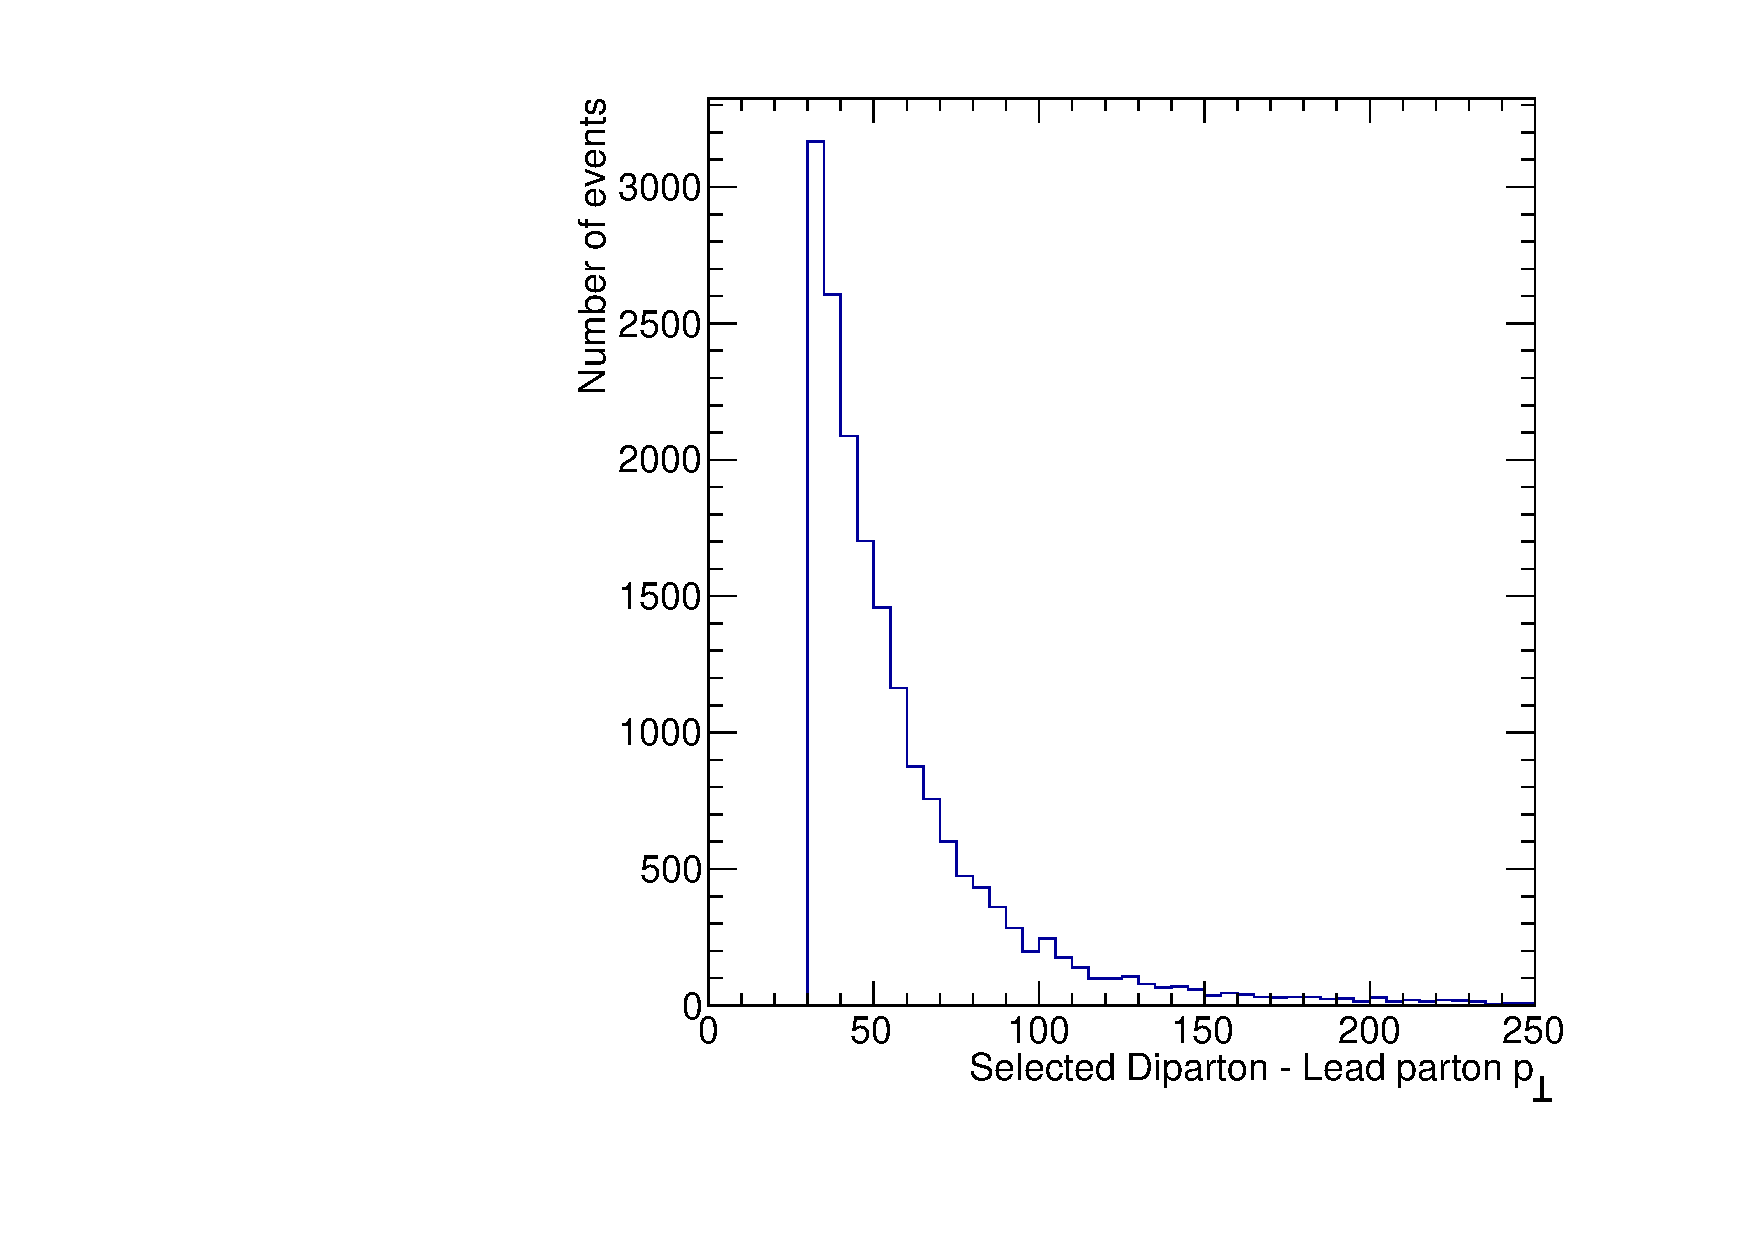
\includegraphics[width=0.8\linewidth]{img/SelDiParton_Parton1_Pt.pdf}
  \end{block}
  
  \column[t]{0.45\linewidth}  
  \centering

  \begin{block}{Sublead Parton $p_\perp$}
    \centering
    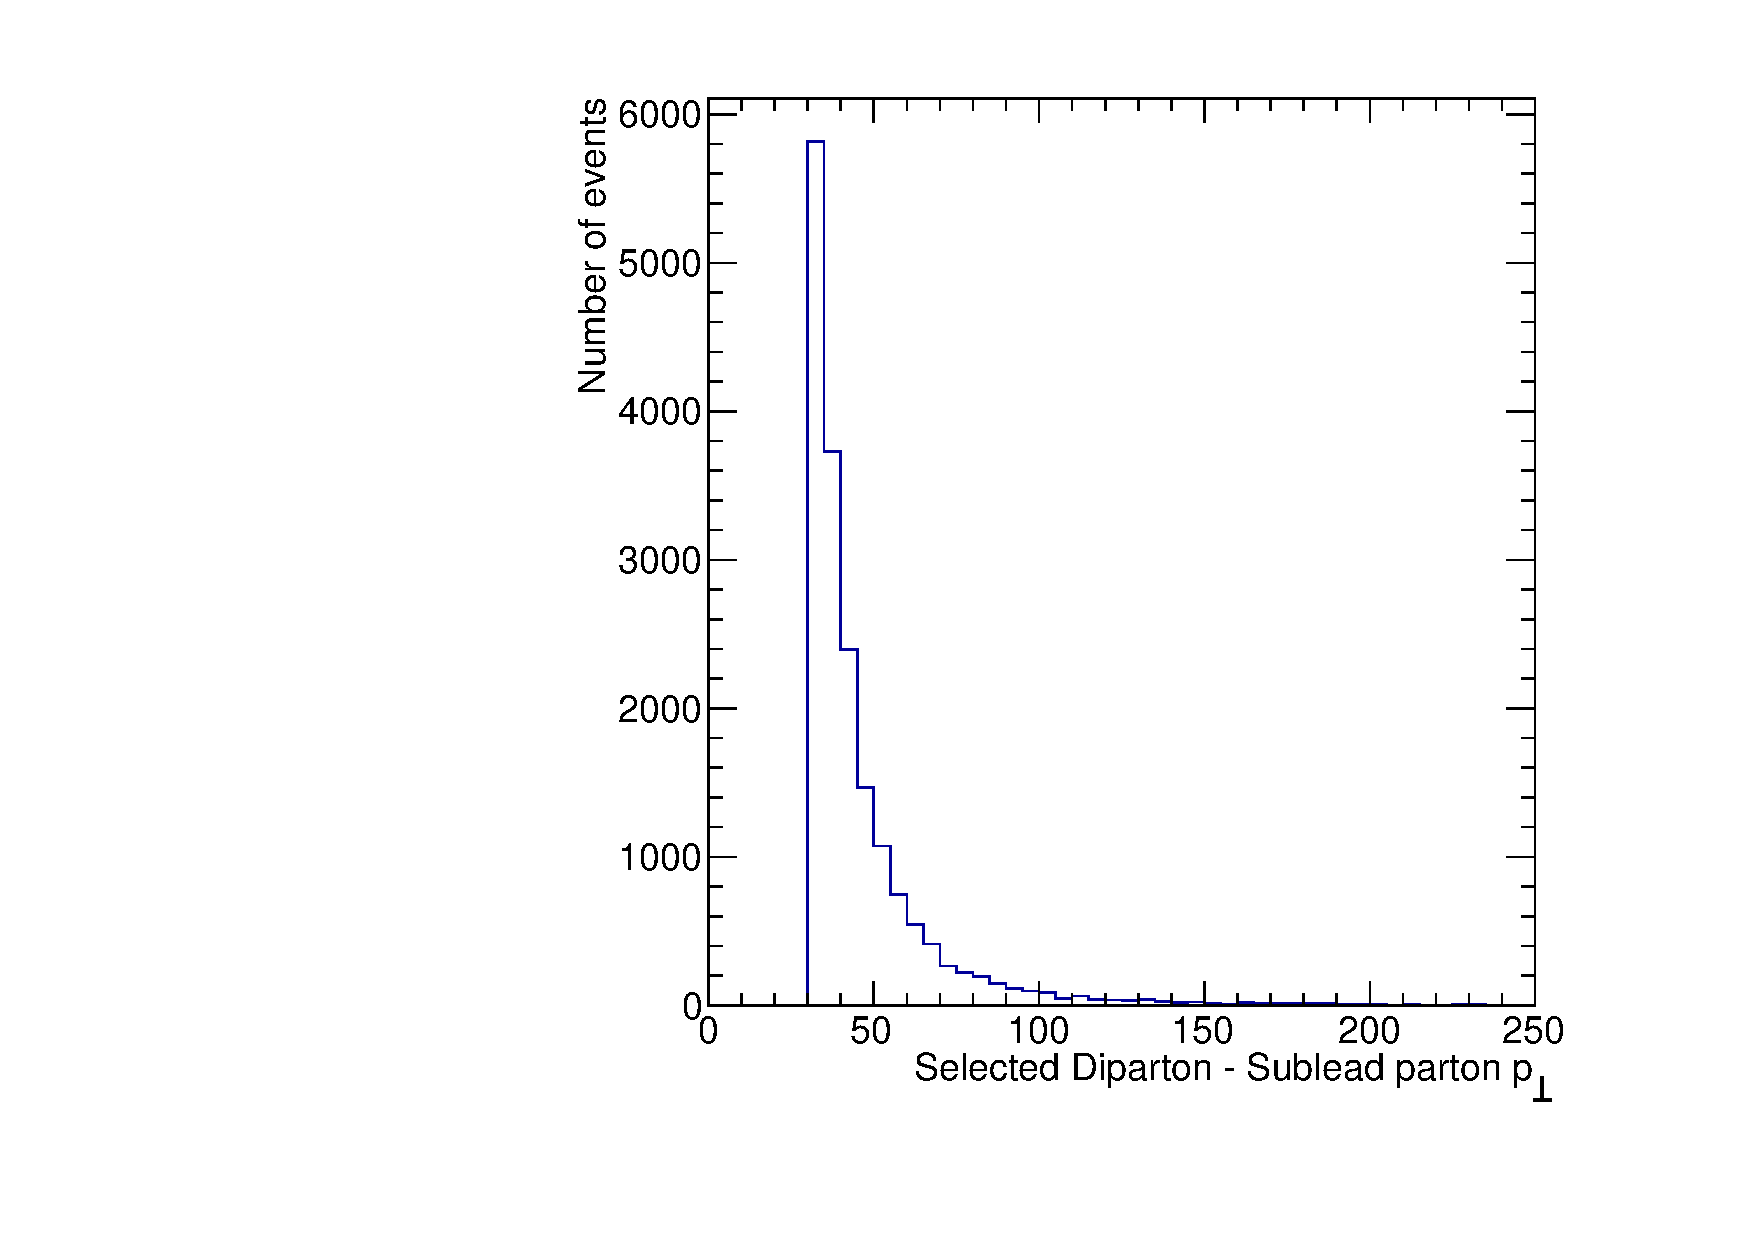
\includegraphics[width=0.8\linewidth]{img/SelDiParton_Parton2_Pt.pdf}
  \end{block}

\end{columns}

\begin{center}
\textbf{Custom MadGraph cuts on dijet parton $p_\perp$ are implemented correctly.}
\end{center}

\end{frame}

% ###################################################
\begin{frame}{Selected Di-parton II}

\begin{columns}

  \column[t]{0.45\linewidth}  
  \centering

  \begin{block}{Lead Parton $p\eta$}
    \centering
    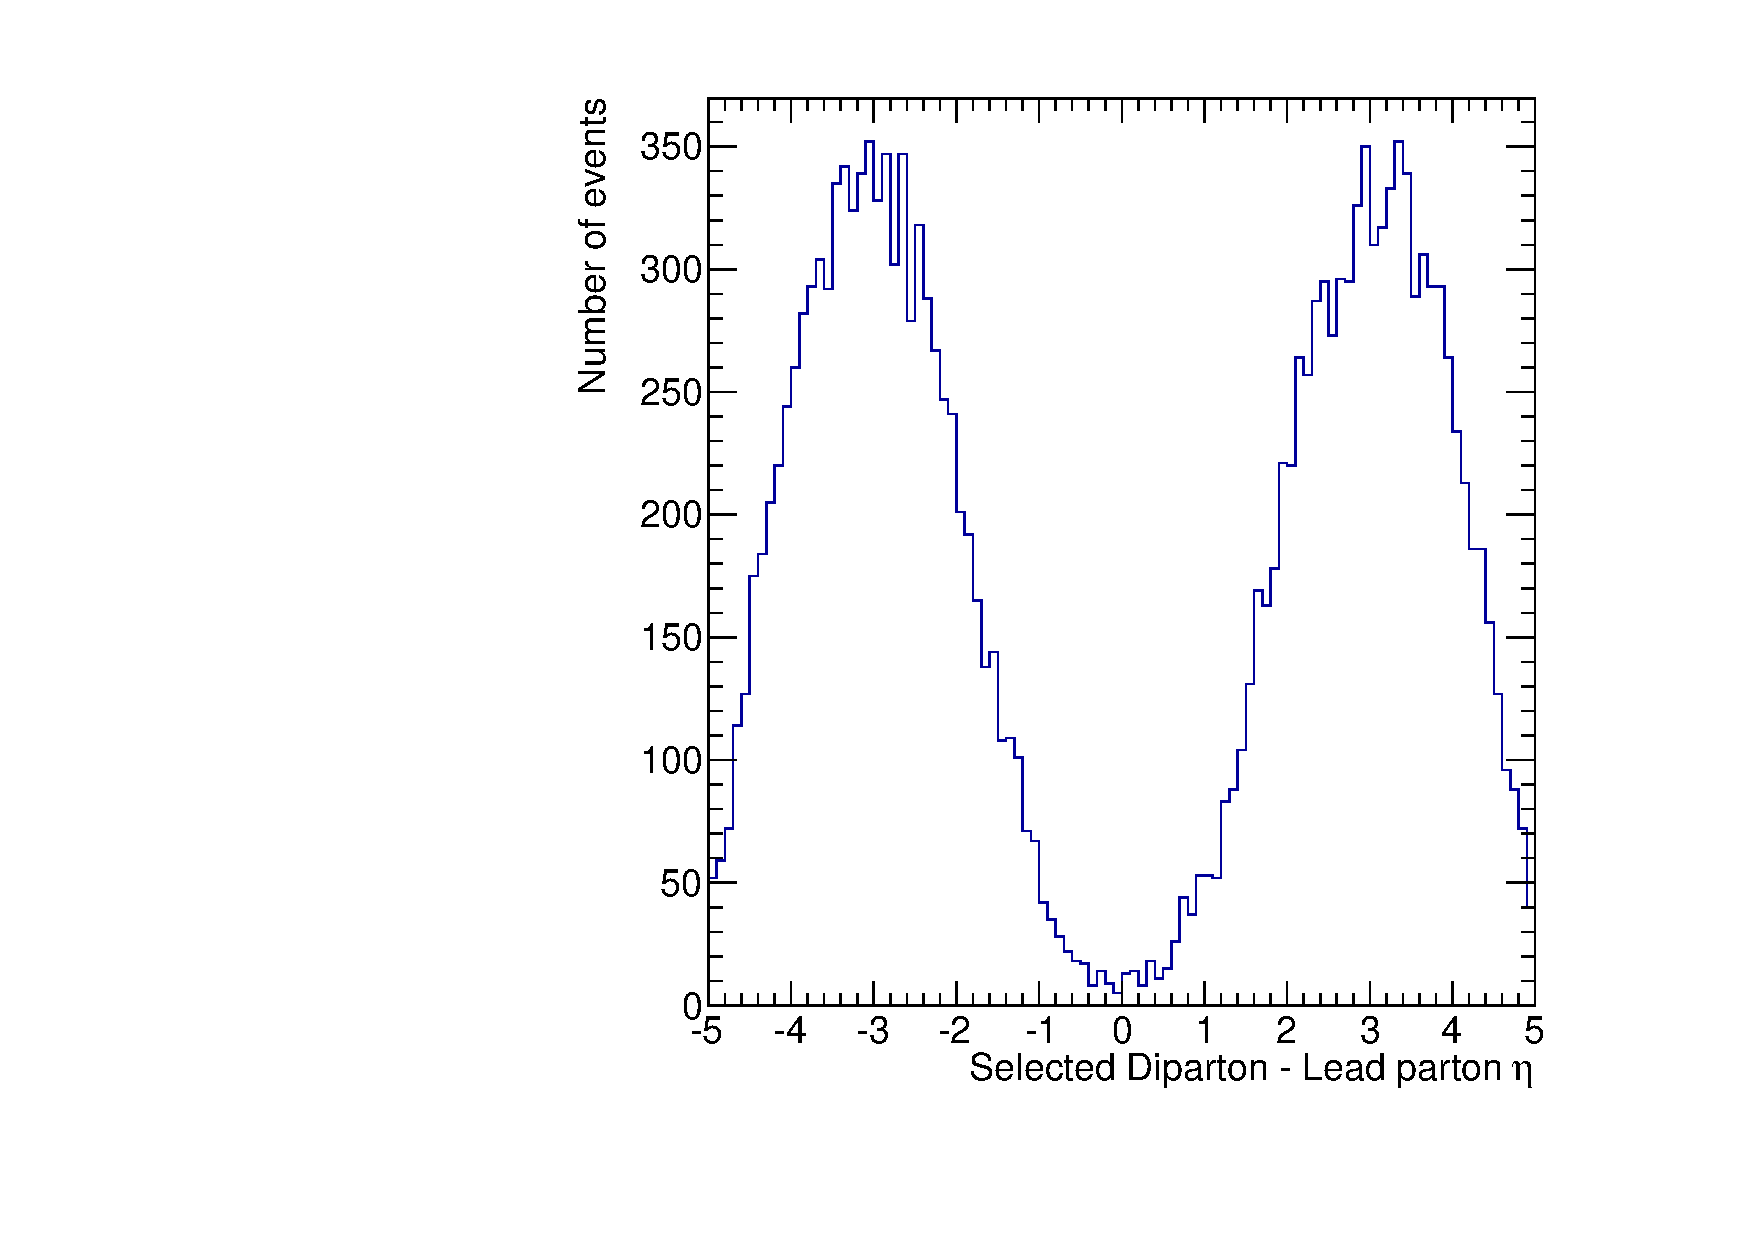
\includegraphics[width=0.8\linewidth]{img/SelDiParton_Parton1_Eta.pdf}
  \end{block}
  
  \column[t]{0.45\linewidth}  
  \centering
 
  \begin{block}{Sublead Parton $\eta$}
    \centering
    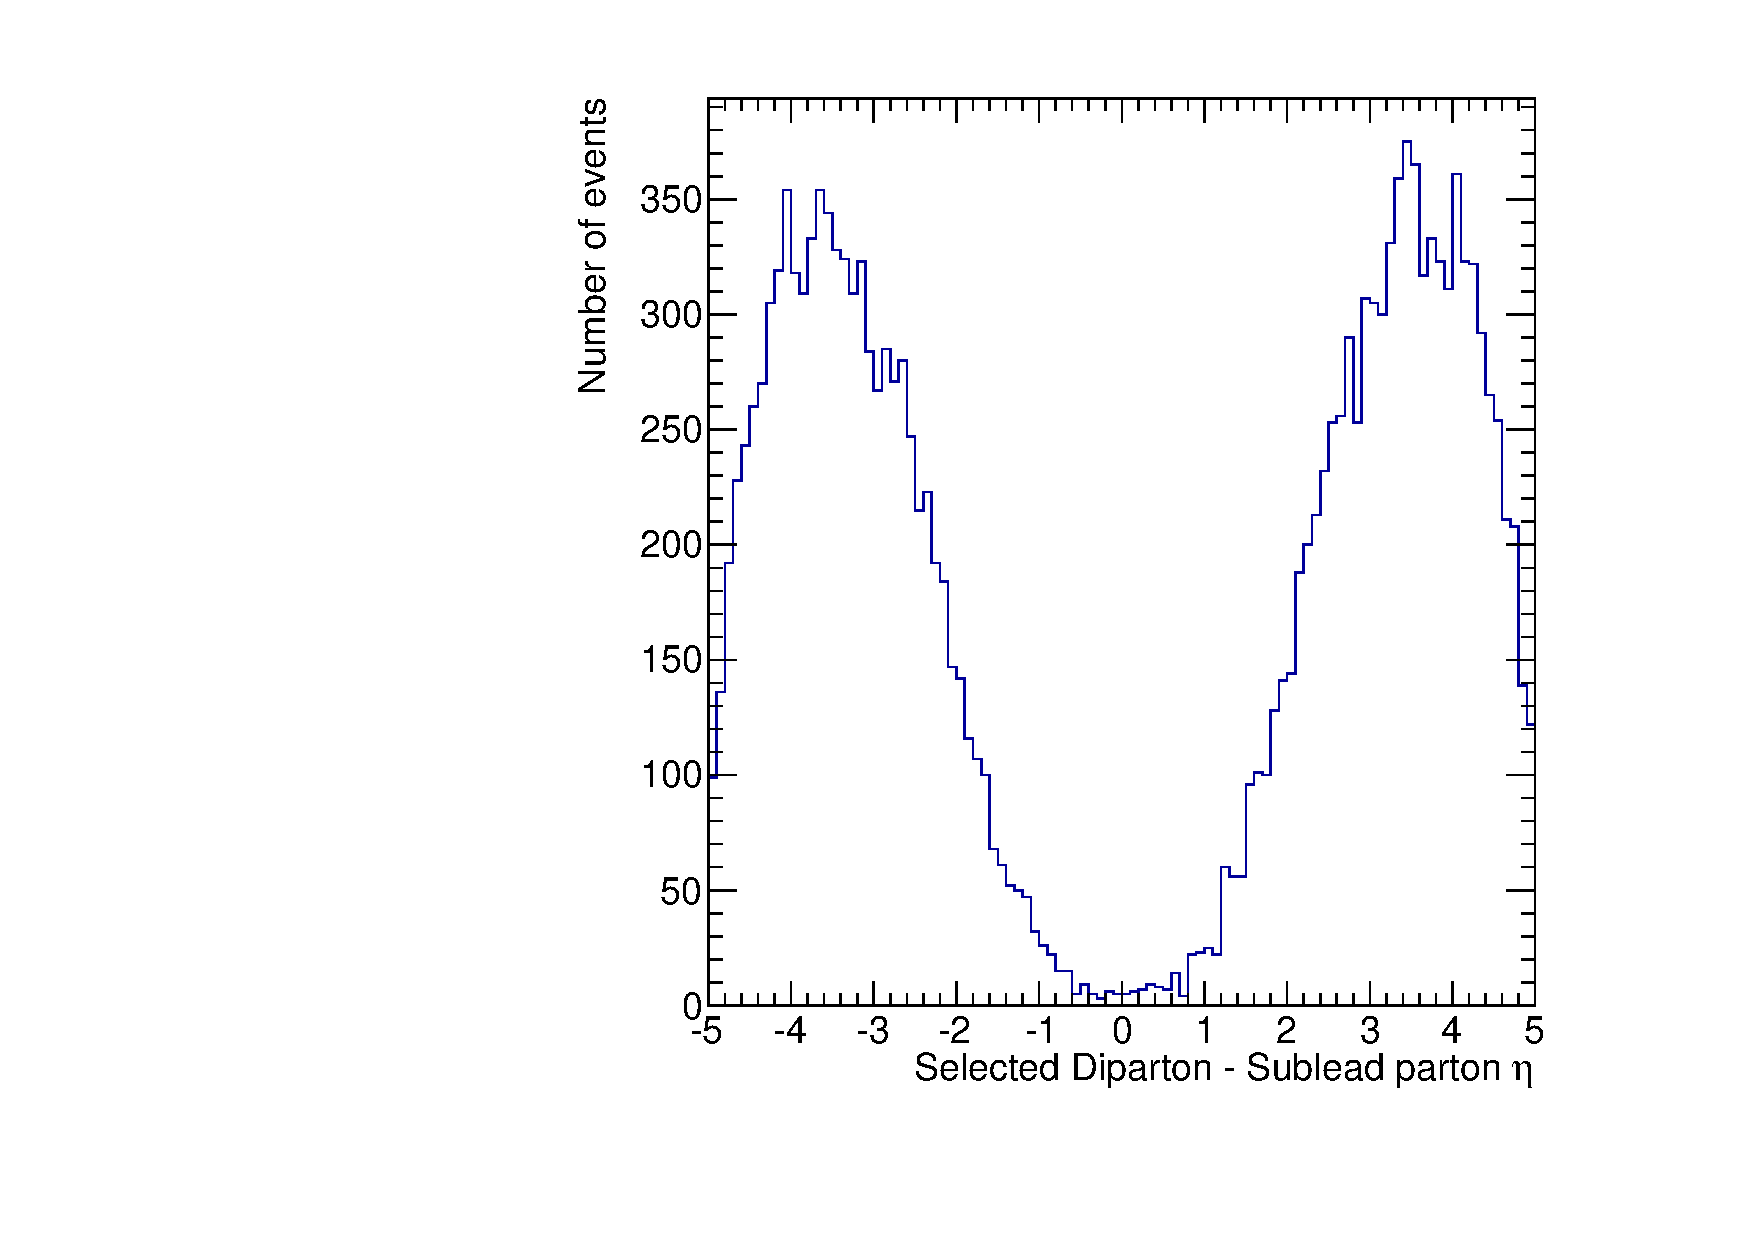
\includegraphics[width=0.8\linewidth]{img/SelDiParton_Parton2_Eta.pdf}
  \end{block}

\end{columns}

\begin{center}
\textbf{Jet $\eta$ distribution looks ok. MadGraph cut is at 5.0.}
\end{center}

\end{frame}

% ###################################################
\begin{frame}{Selected Di-parton III}

\begin{columns}

  \column[t]{0.45\linewidth}  
  \centering

  \begin{block}{Di-parton $\Delta\eta$}
    \centering
    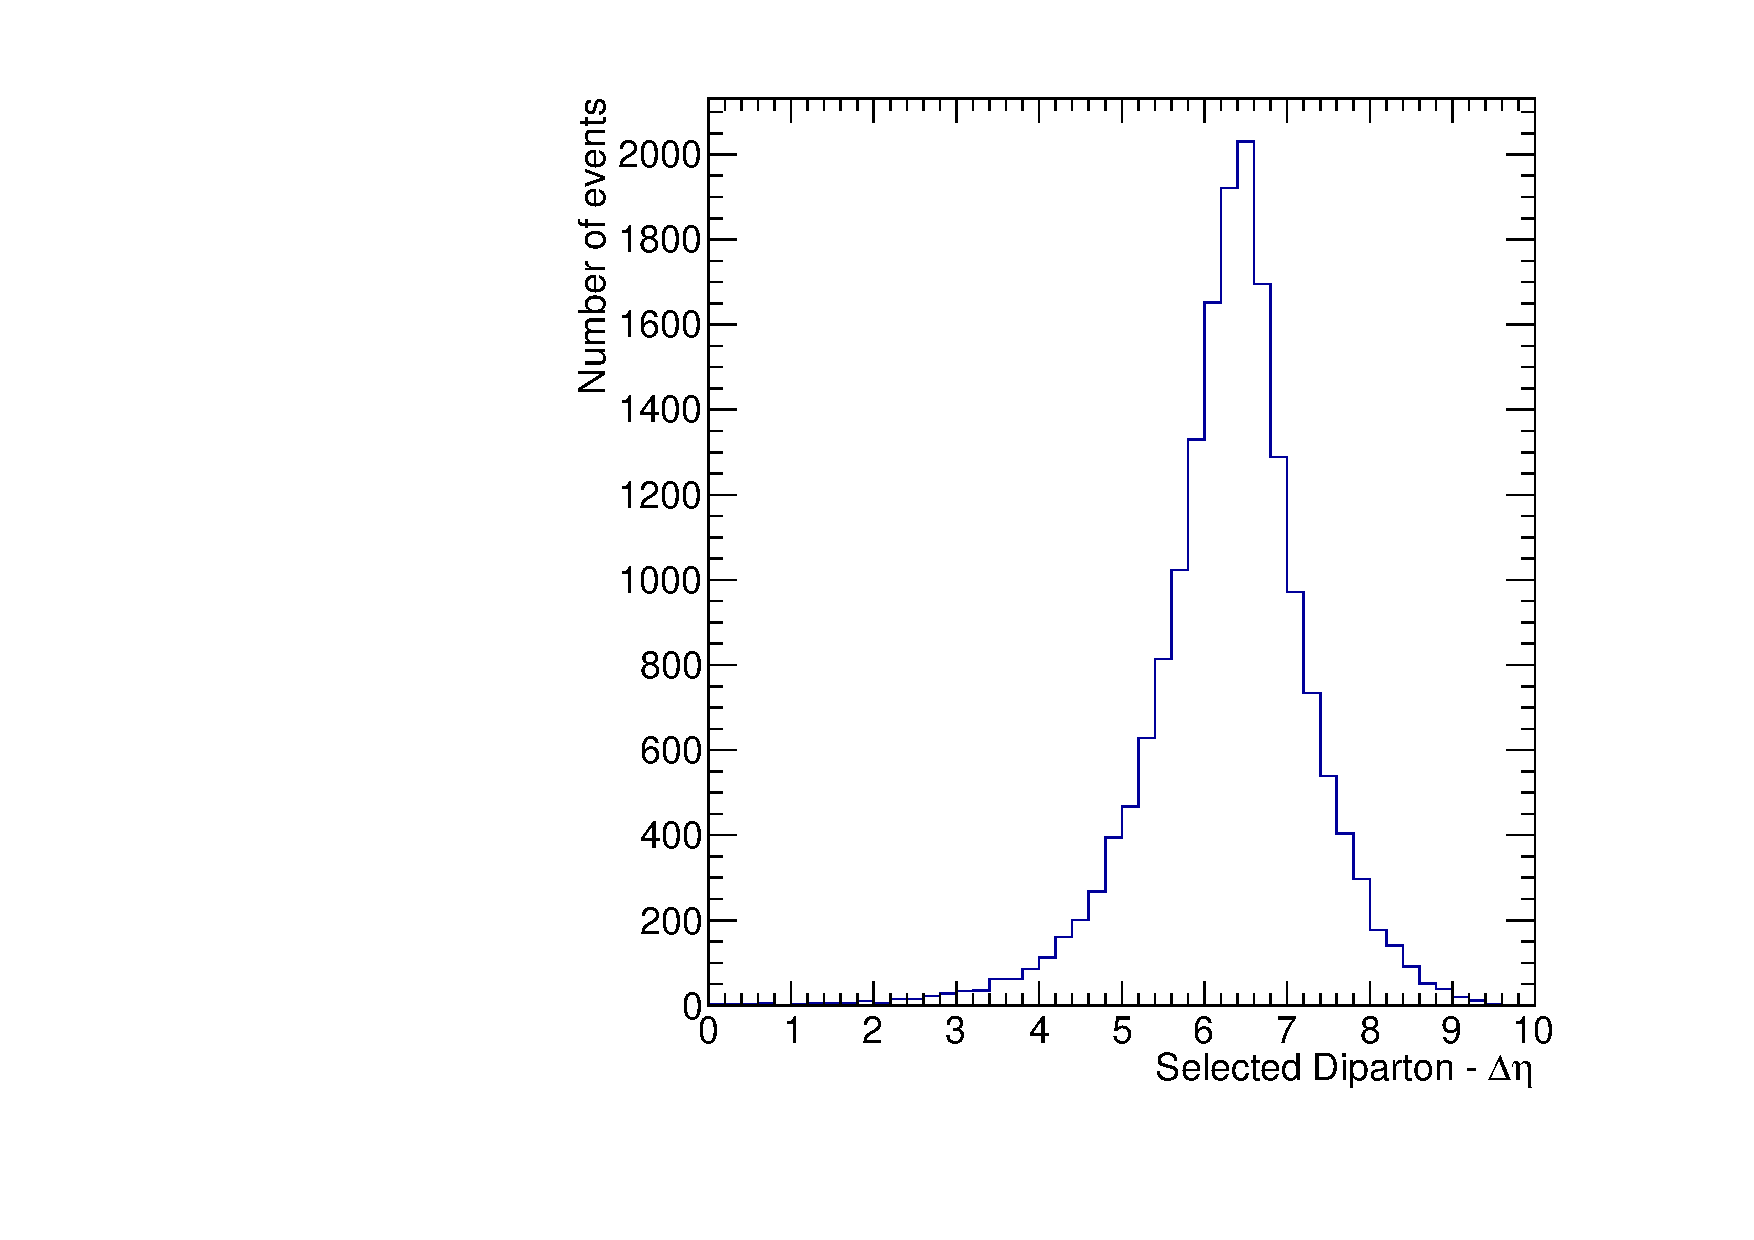
\includegraphics[width=0.8\linewidth]{img/SelDiParton_DEta.pdf}
  \end{block}
  
  \column[t]{0.45\linewidth}  
  \centering
 
  \begin{block}{Di-parton $m_{jj}$}
    \centering
    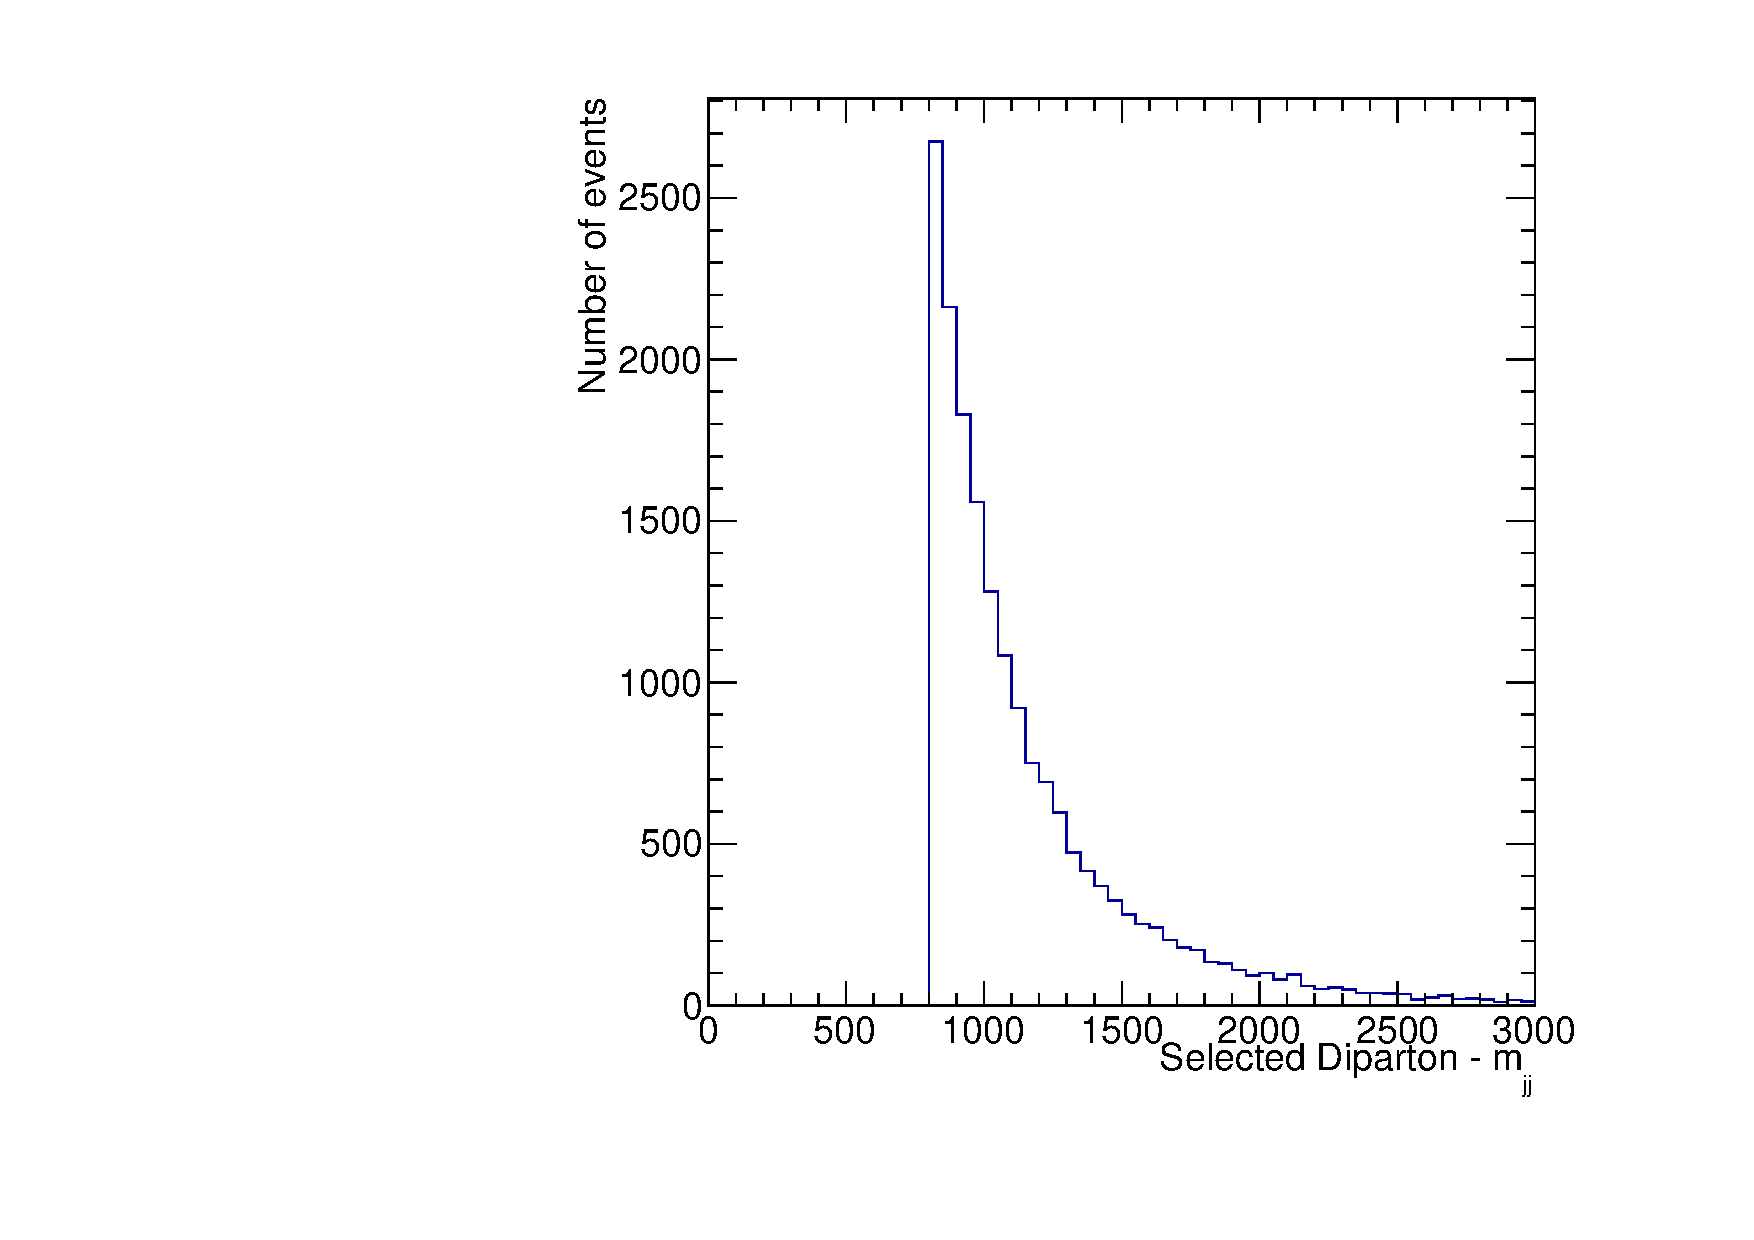
\includegraphics[width=0.8\linewidth]{img/SelDiParton_Mjj.pdf}
  \end{block}

\end{columns}

\begin{center}
\textbf{Custom MadGraph cuts on dijet parton $m_{jj}$ are implemented correctly. $\Delta\eta$ peaks over 6 showing that this variable indeed could not be used to reduce QCD.}
\end{center}

\end{frame}

% ###################################################
\begin{frame}{Parton-Generator Jet Matching procedure}

\begin{block}{Pairing Partons and Generator Jets}

\begin{itemize}
  \item Selecting all generator jets within $\Delta R < 0.4$ 
  \item From those selecting the generator jet with the lowest $p_\perp$ to the parton as a match.
  \begin{itemize}
    \item This avoids picking up the wrong jet from just picking lowest $\Delta R$
  \end{itemize}
\end{itemize}

\end{block}

\begin{block}{Results}
  
\begin{center}
  

\begin{tabular}{|c||c|c|c||c|}
\hline
            &          \multicolumn{4}{c|}{Process} \\
\hline
$n_{match}$ &      jj &    jjj  &    jjjj &   Total \\
\hline\hline 
          0 & 03.54\% &  0.29\% & 00.05\% & 01.53\% \\
          1 & 25.21\% &  4.23\% & 01.35\% & 11.80\% \\
          2 & 71.25\% & 27.55\% & 08.66\% & 39.11\% \\
          3 &         & 67.92\% & 36.16\% & 29.98\% \\
          4 &         &         & 53.77\% & 17.58\% \\
\hline
\end{tabular}

\end{center}

\begin{itemize}
  \item Selected diparton has a match     : 73.96\%
  \item Generator jet matched not lowest $\Delta R$ :  3.57\%
\end{itemize}

\end{block}

\begin{center}
\textbf{With the current matching procedure we can find matches for the selected di-parton most of the times.}
\end{center}

\end{frame}

% ###################################################
\begin{frame}{Selected Di-partons vs Matched Generator Jet I}

\begin{columns}

  \column[t]{0.45\linewidth}  
  \centering

  \begin{block}{Lead Parton-Generator Jet $p_\perp$}
    \centering
    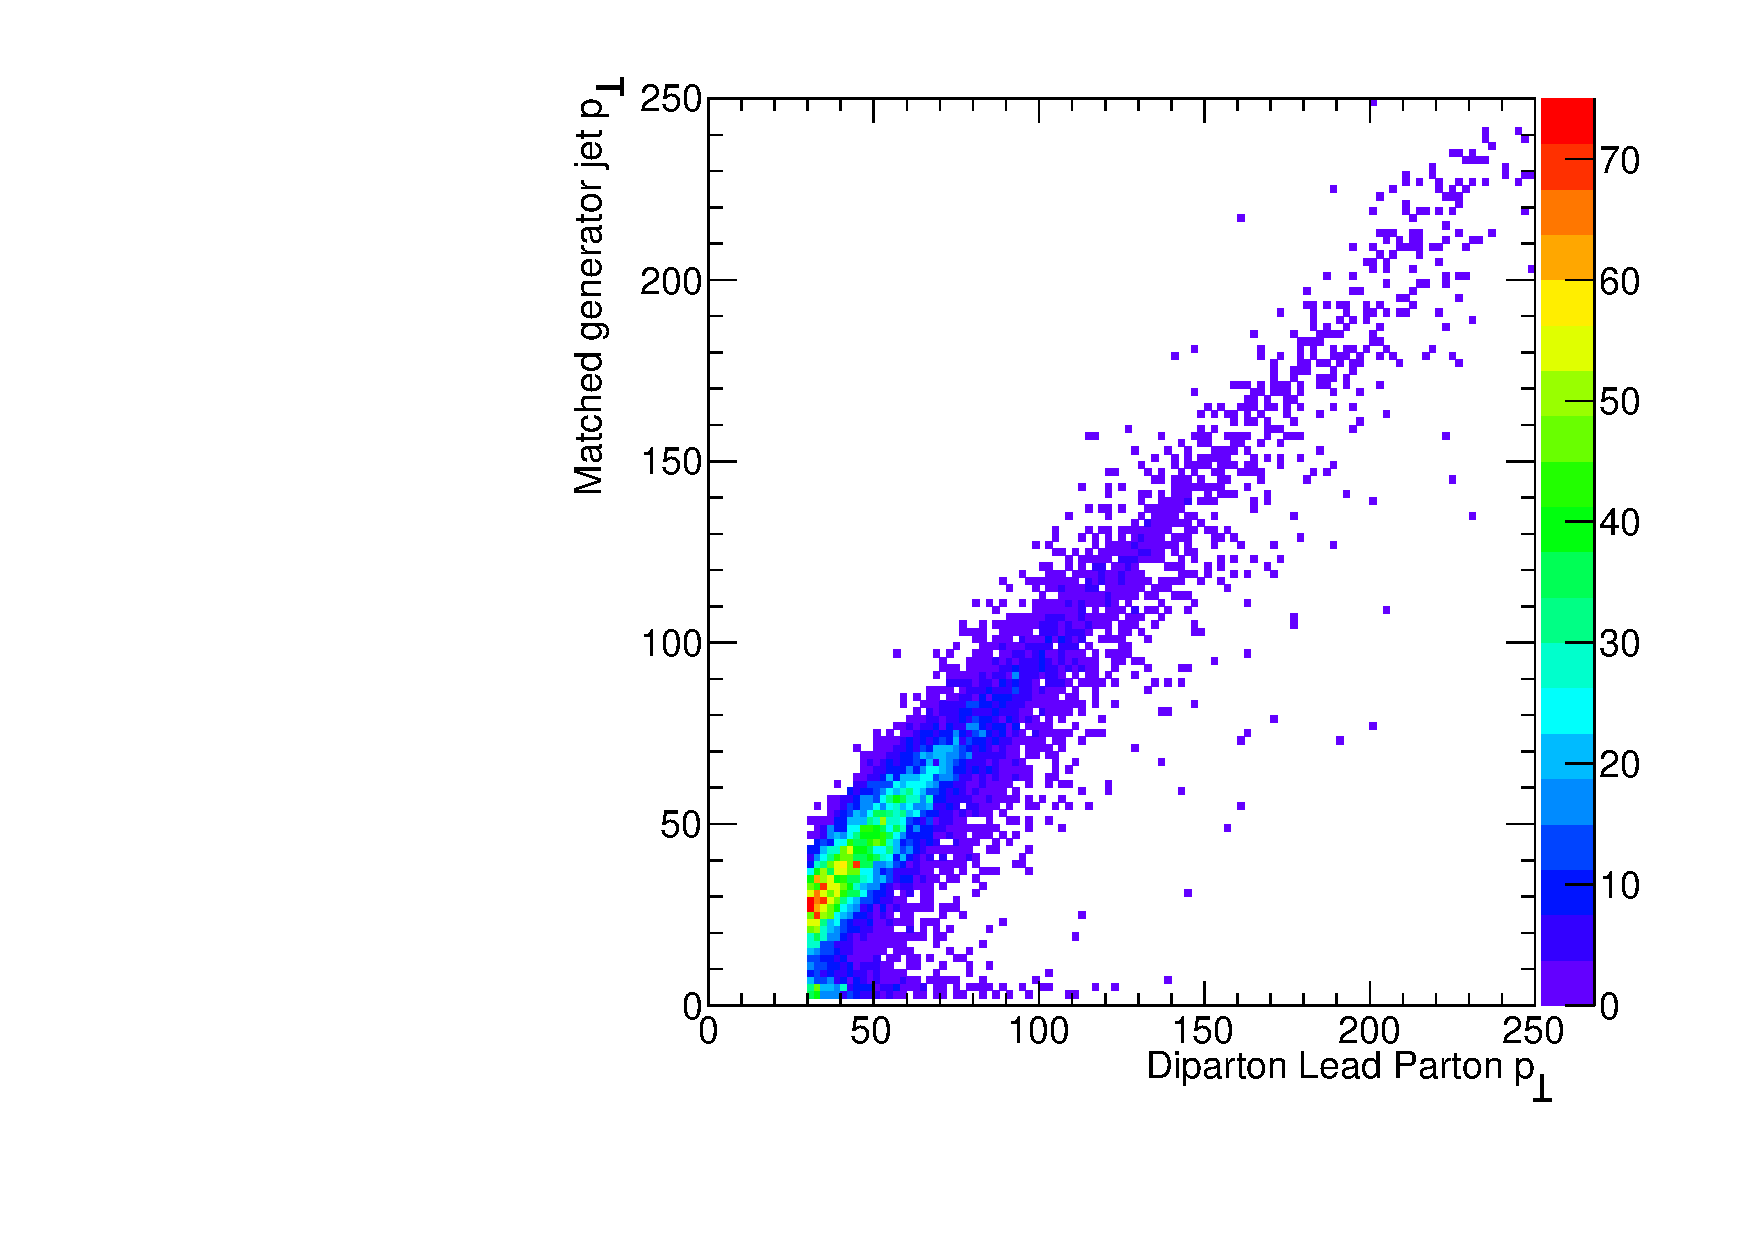
\includegraphics[width=0.8\linewidth]{img/SelDiParton_MatchedGenJet_Parton1_Pt.pdf}
    
  \end{block}
  
  \column[t]{0.45\linewidth}  
  \centering
 
  \begin{block}{Sublead Parton-Generator Jet $p_\perp$}
    \centering
    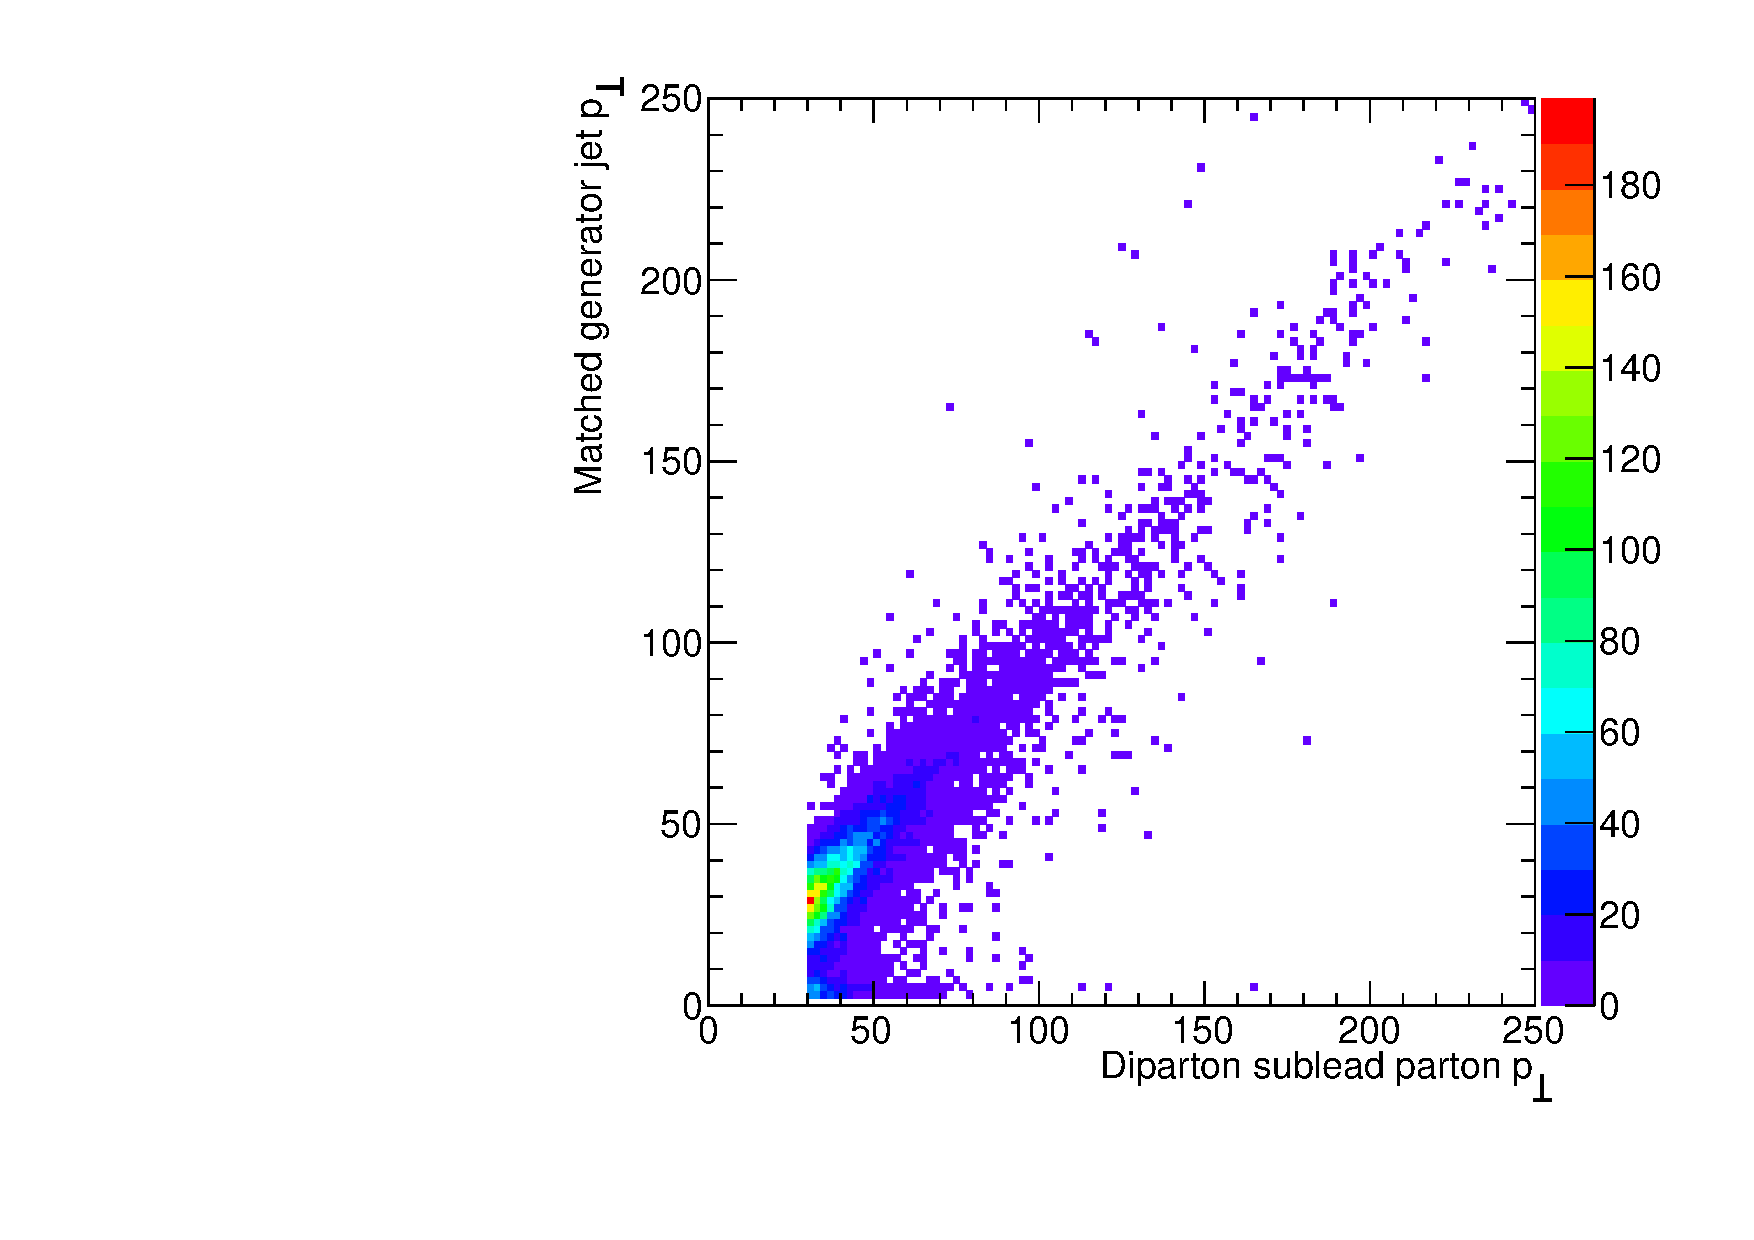
\includegraphics[width=0.8\linewidth]{img/SelDiParton_MatchedGenJet_Parton2_Pt.pdf}
  \end{block}

\end{columns}

\begin{itemize}
  \item \tiny{Lead jets: In the bin Parton $30<p_\perp\leq32$ GeV only $2.04\% \pm 0.54\%$ generator jets are $p_\perp\geq40$ $GeV$}
  \item \tiny{Sublead jets: In the bin Parton $30<p_\perp\leq32$ GeV only $3.34\% \pm 0.49\%$ generator jets are $p_\perp\geq40$ $GeV$}
\end{itemize}

\begin{center}
\textbf{Parton to generator jet $p_\perp$ migration are under 3.5\% at the bin $30<p_\perp\leq32$ and should be even lower at $p_\perp<30$. This is acceptable.}
\end{center}

\end{frame}

% ###################################################
\begin{frame}{Selected Di-partons vs Matched Generator Jet II}

\begin{columns}

  \column[t]{0.45\linewidth}  
  \centering

  \begin{block}{Lead Parton-Generator Jet $\eta$}
    \centering
    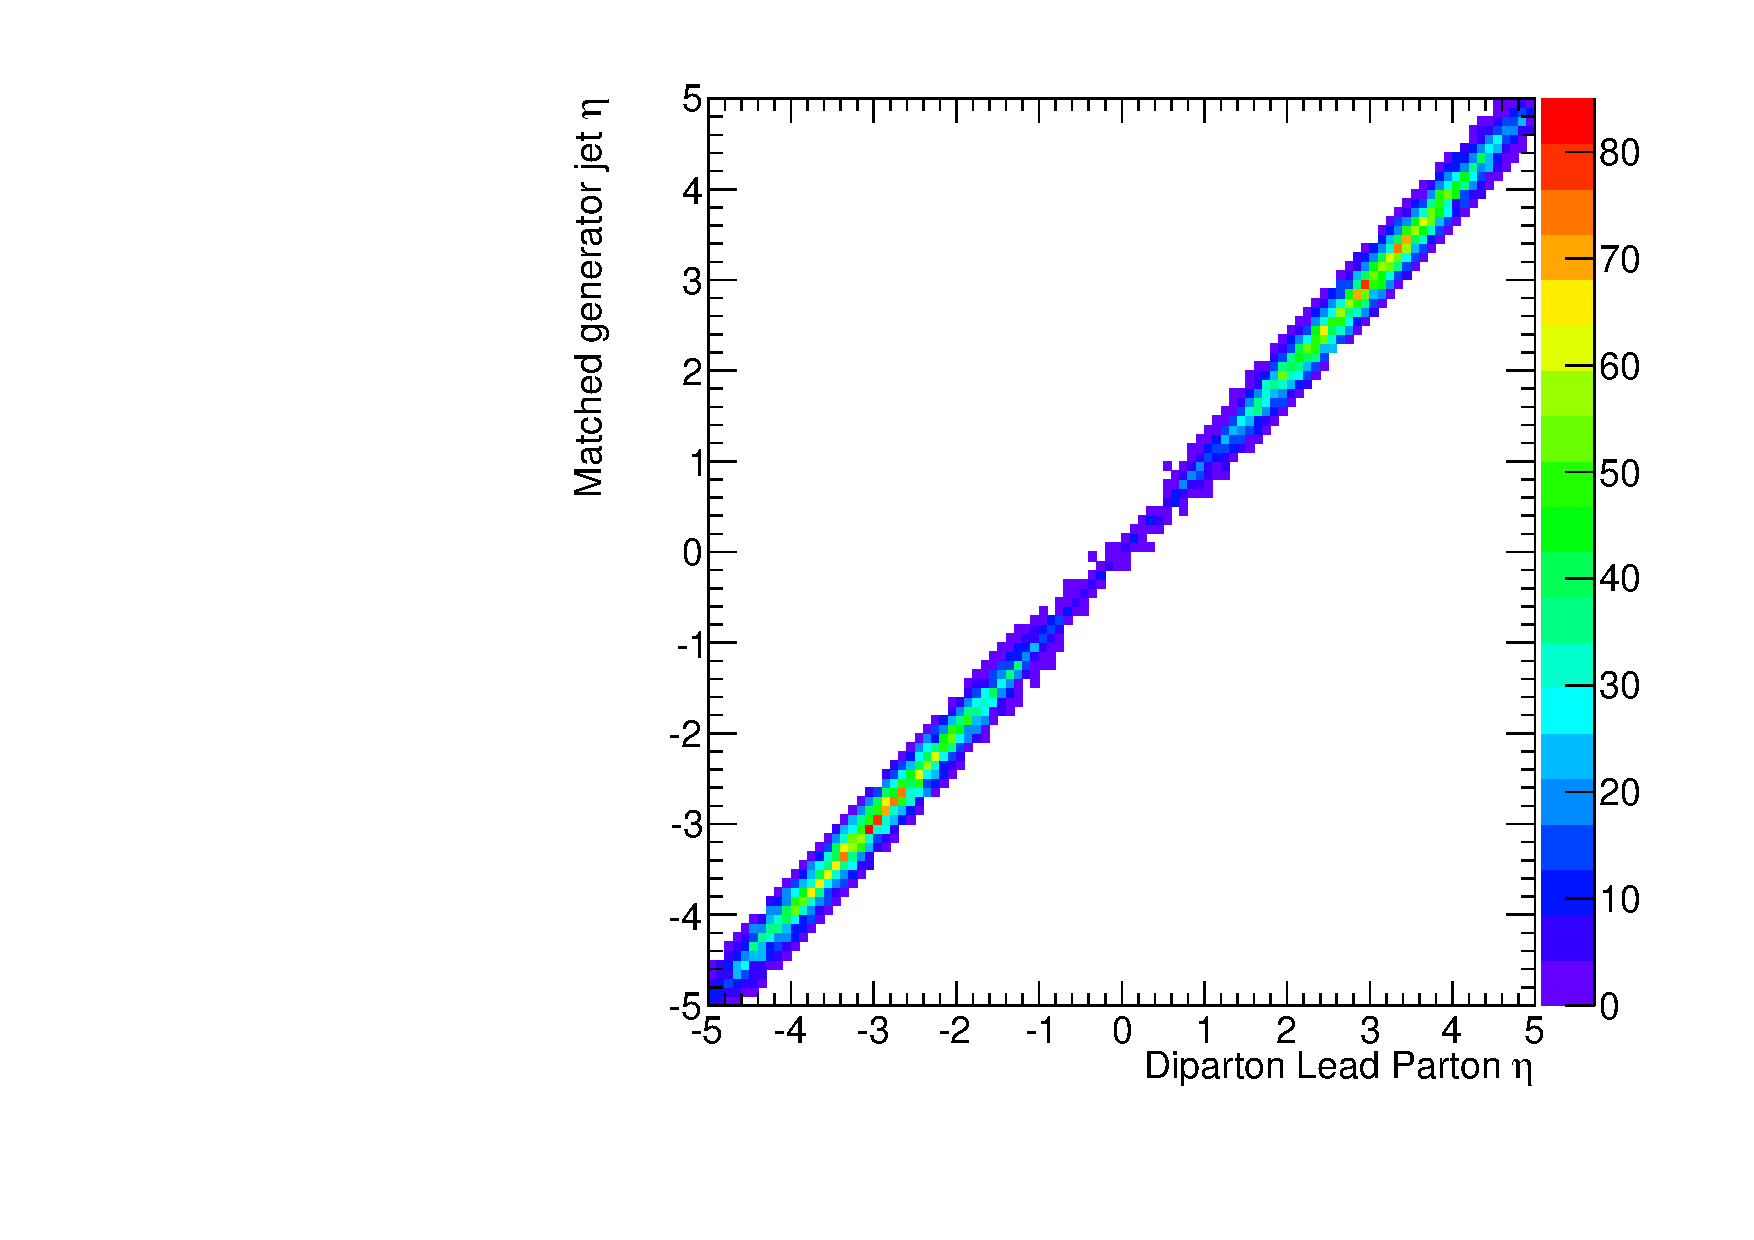
\includegraphics[width=0.8\linewidth]{img/SelDiParton_MatchedGenJet_Parton1_Eta.pdf}
  \end{block}
  
  \column[t]{0.45\linewidth}  
  \centering
 
  \begin{block}{Sublead Parton-Generator Jet $\eta$}
    \centering
    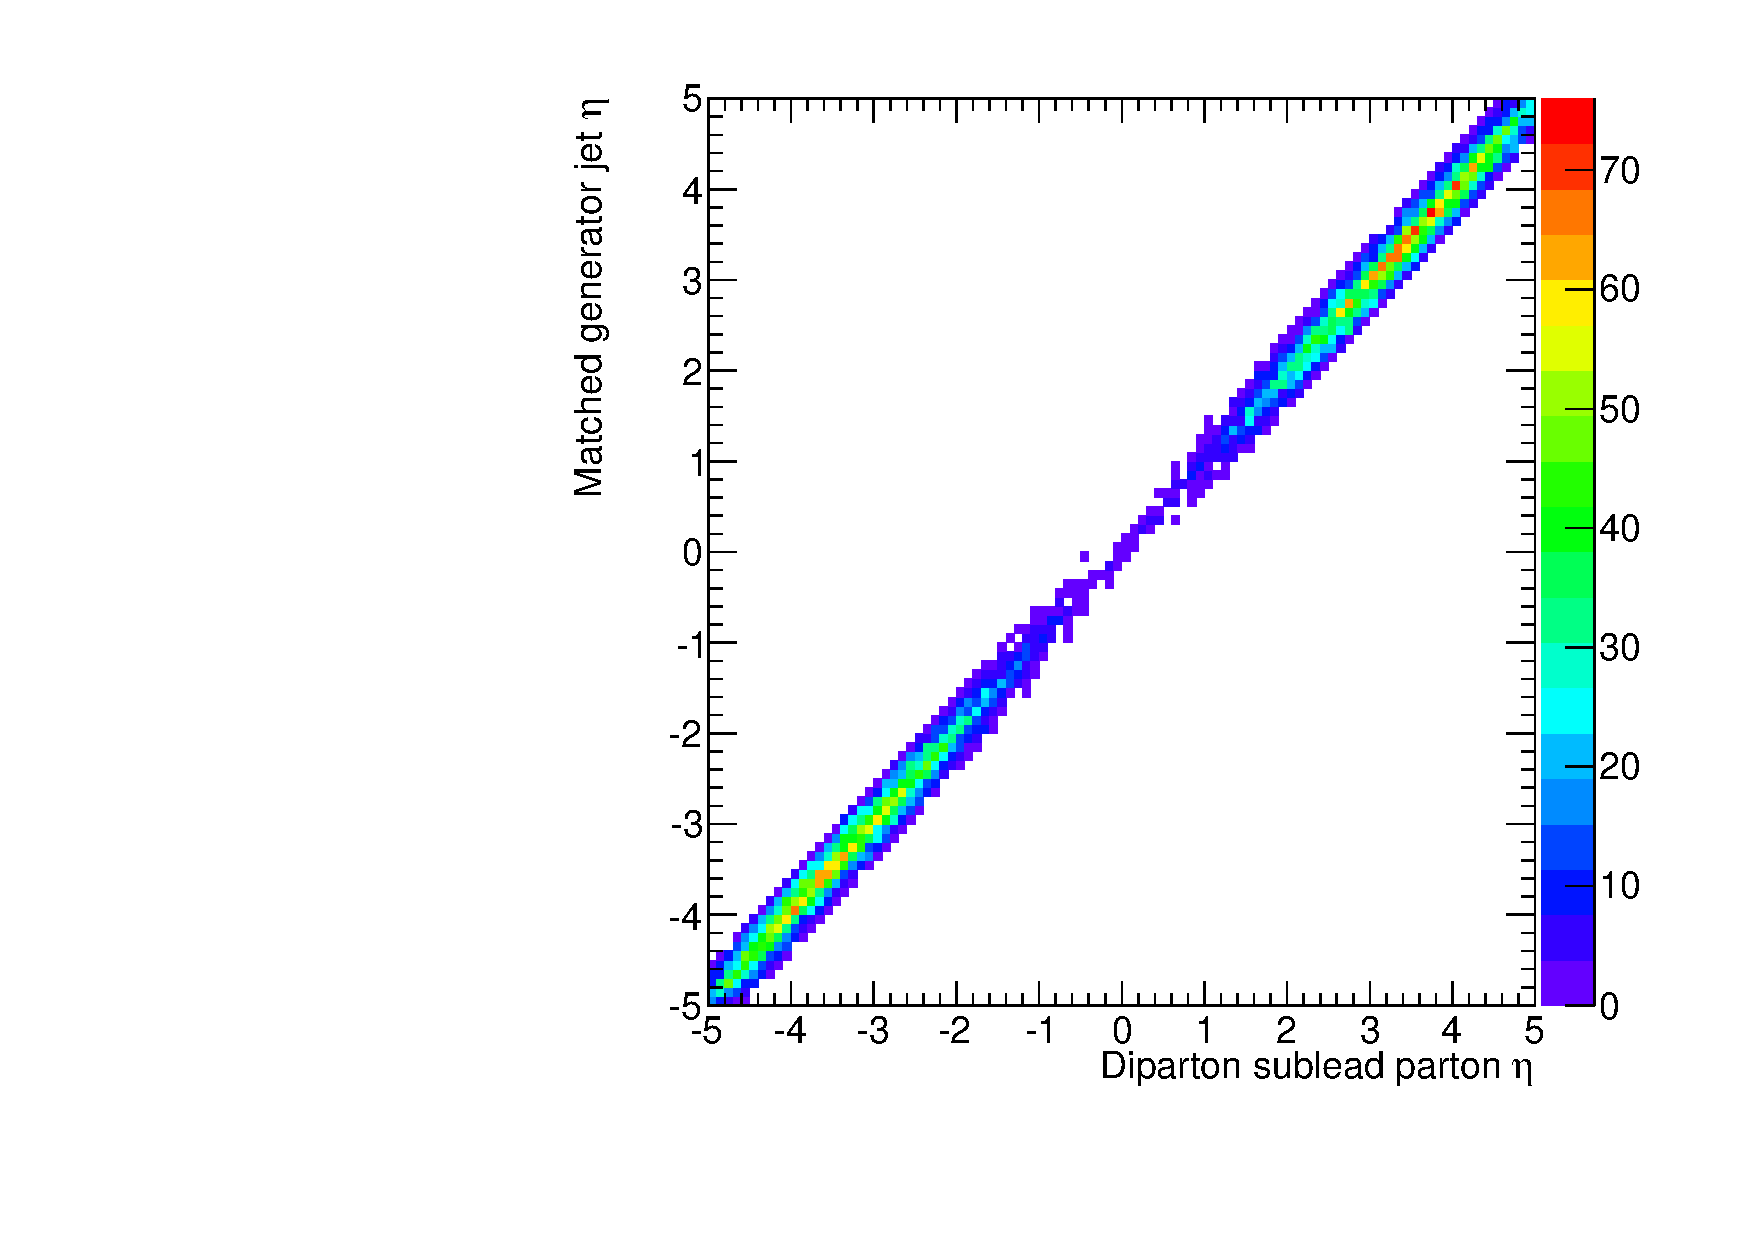
\includegraphics[width=0.8\linewidth]{img/SelDiParton_MatchedGenJet_Parton2_Eta.pdf}
  \end{block}

\end{columns}

\begin{center}
\textbf{Parton to generator jet $\eta$ migration are in general under 0.5.}
\end{center}

\end{frame}

% ###################################################
\begin{frame}{Selected Di-partons vs Matched Generator Jet III}

\begin{columns}

  \column[t]{0.45\linewidth}  
  \centering

  \begin{block}{Di-parton-Generator Dijet $\Delta\eta$}
    \centering
    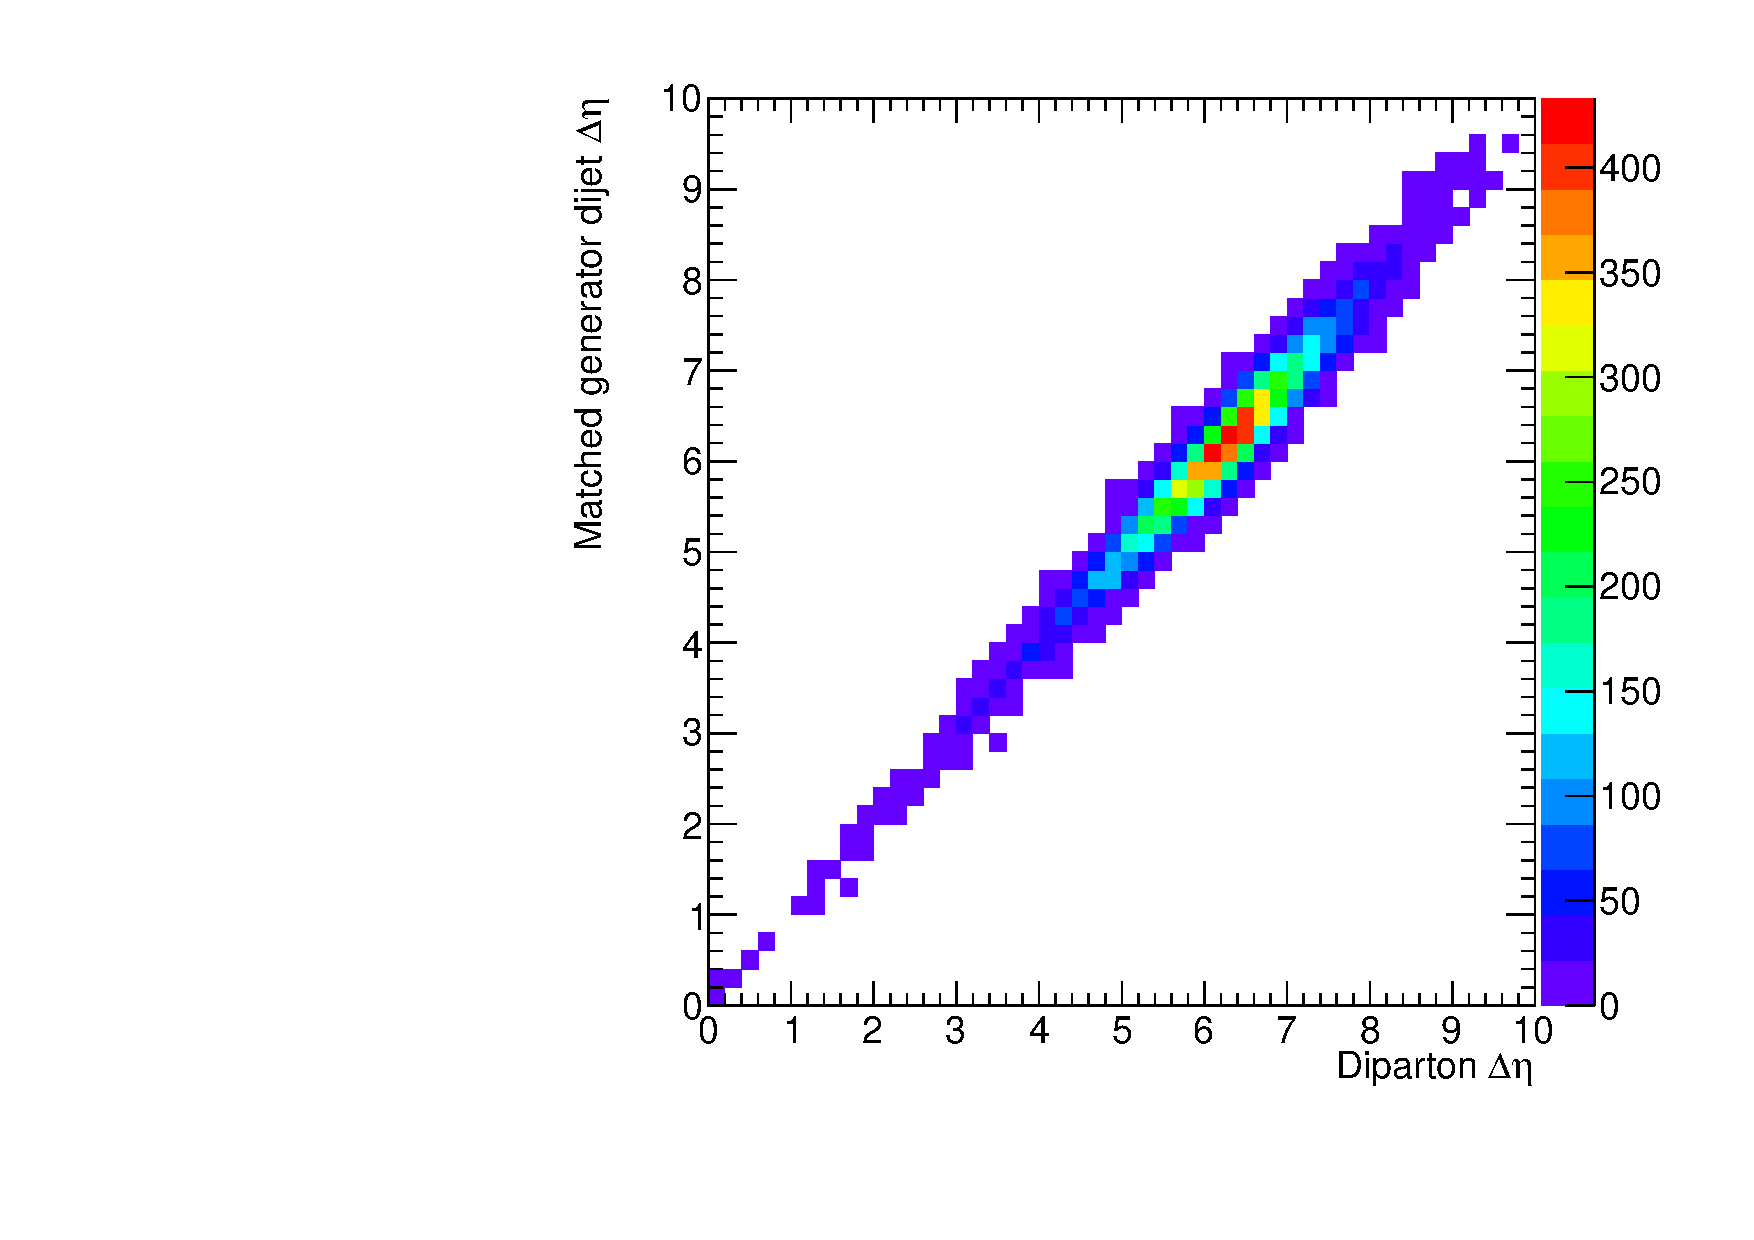
\includegraphics[width=0.8\linewidth]{img/SelDiParton_MatchedGenJet_DEta.pdf}
  \end{block}
  
  \column[t]{0.45\linewidth}  
  \centering
 
  \begin{block}{Di-parton-Generator Dijet $m_{jj}$}
    \centering
    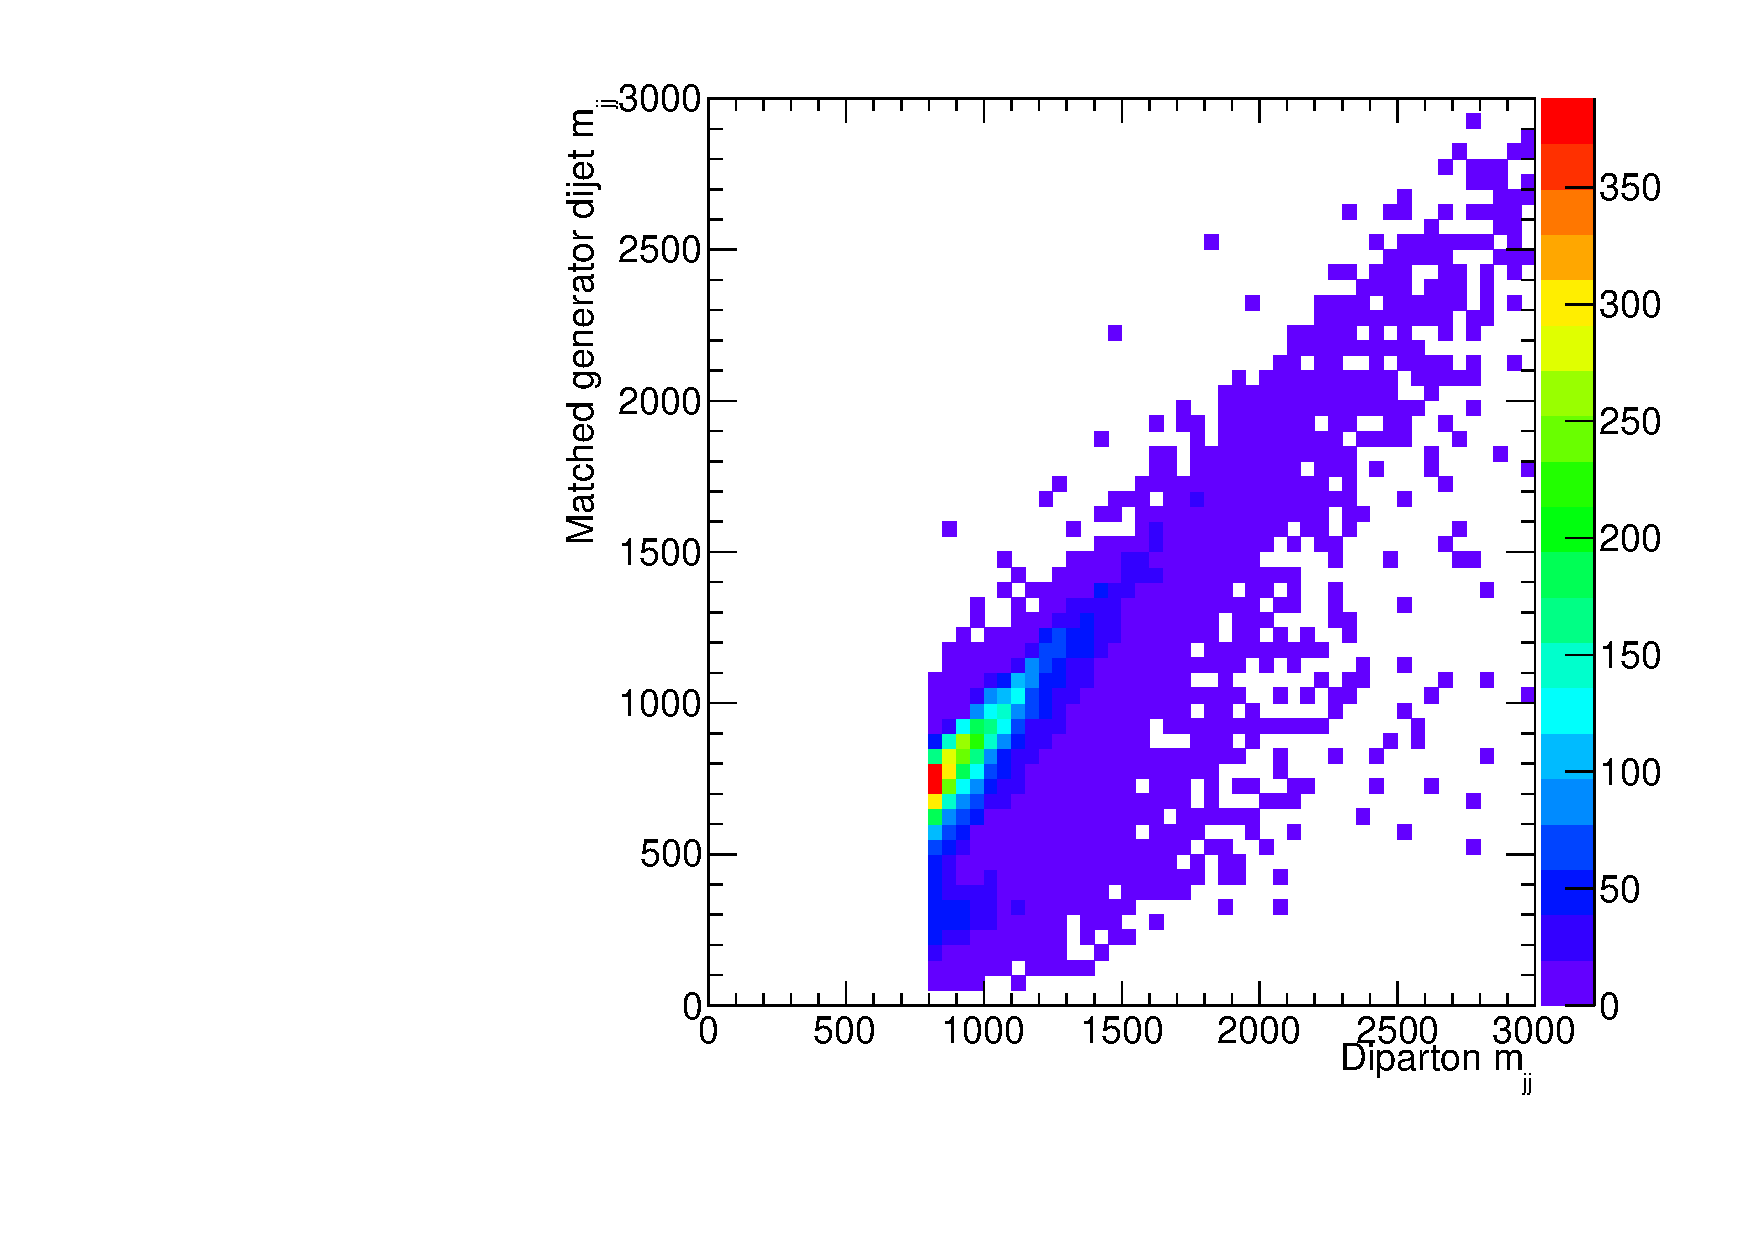
\includegraphics[width=0.8\linewidth]{img/SelDiParton_MatchedGenJet_Mjj.pdf}
  \end{block}

\end{columns}

\begin{itemize}
  \item \tiny{$m_{jj}$: In the bin Di-parton $800<m_{jj}\leq850$ GeV only $1.09\% \pm 0.23\%$ generator dijets are $m_{jj}\geq900$ $GeV$}
\end{itemize}

\begin{center}
\textbf{Migration in dijet $m_{jj}$ are very small even at 900 $GeV$.}
\end{center}

\end{frame}

% ###################################################
\begin{frame}{Conclusions}

\begin{block}{Summary}
  
\begin{itemize}
  \item A MadGraph gridpack was produce following the CMS Generator Group recommended instructions
  \item A test run was made producing 185k events where it was demonstrated that the custom proposed cuts were correctly implemented.
  \item Pythia8 hadronization was performed over the parton level events with an efficiency of $ 9.7 \pm 0.1$ and leading to a final sample cross section of $9.828e+05 \pm 7.440e+03$.
  \item A study over the key variable migration was performed showing that they are acceptable for the proposed generator level filter.
  \item We are ready to pass this gridpack to the generator group and request our new QCD sample production.
\end{itemize}
  
\end{block}

\end{frame}

\end{document}
